\section{Testing Framework}
\label{sec:testing Framework}
Im folgenden Kapitel werden wir auf die einzelnen Komponenten des von uns entwickelten Test Frameworks eingehen und die Funktionsweise erläutern. Die Aufgabe des Test Framework liegt darin, die verschiedenen Prototypen, welche im Laufe dieser Semesterarbeit entwickelt wurden, mit dieses Framework einheitlich testen zu lassen. Das Test Framework wurde parallel zum RMIOnly- Systems mit Concurrency Control entwickelt.

\subsection{Konzept}
Das Framework lässt sich über eine Konfigurationsdatei konfigurieren und kann Testfälle die in einer XML Datenstruktur vorliegen intepretieren und daraus die einzelnen Testszenarien generieren. Die Testszenarien werden vom Server auf die verfügbaren Testframework Clients verteilen und dort gestartet, hat ein Testframework Client ein Szenario auf einem ClientSystemUnderTest abgearbeitet, wird das Szenario mit den Messwerten zurück an den Server geschickt. Auf dem Server werden dann die Messresultate jedes Szenario ausgewertet und abgespeichert. Dadurch lassen sich die Resultate der verschieden System zu einem späteren Zeitpunkt vergleichen.

\subsection{Open Points (TODO's)}
\begin{itemize}	
\item Netzwerk Traffic der im Zimmer Auftritt kann nicht kontrolliert werden. Messungen daher nicht verlässlich, man bäuchte ein eigenes Netz.
\item JVM Profiler: Beweis für die Zombie Objekte in der JVM, soll das gemacht werden?
\item Logger
\item Exception Handling
\end{itemize}



\subsection{Der Frameworkserver}
\label{sec:test-FW Server}
\subsubsection{Das Startup-Script}
\label{sec:startupScript}
Das  Startup-Script ist ein Shell-Script in der Bash-Sprache geschrieben. Das Script führt mehrere Methoden nacheinander aus:
\begin{enumerate}
\item Das Script prüft die in der Config-Datei eingetragenen Zielrechner auf bereits vorhandene "client.jar"-Dateien und löscht diese Dateien, falls vorhanden
\item Durch die Applikation "Secure Copy" wird die zuvor im Buildprozess erstellte Datei "client.jar" auf die Zielrechner kopiert
\item Via SSH wird der Frameworkclient auf den Zielrechnern gestartet
\item Der Frameworkserver wird gestartet
\end{enumerate}
Sind diese Schritte abgeschlossen, beendet das Startupscript und die weitere Ausführung des Testlaufs wird durch den Frameworkserver orchestriert.
Beim Starten des Scripts wird der Name der Datei mitgegeben, in welcher der genaue Testlauf definiert ist. Wird kein Argument mitgegeben, läuft der Standardtestlauf ab, welcher in der Datei "testCases.xml" beschrieben ist.
Probleme beim Schreiben des Scripts waren selten. Ein Problem, welches gelöst werden musste war der Umstand, dass das Script nach dem Starten eines Clients nicht mehr weiterlief, sondern einfach wartete. Dies war bei folgende Zeile der Fall:
\begin{lstlisting}	
 ssh student@${i} "java -jar ${remotePath}/${clientJar}"
\end{lstlisting}	
Offensichtlich wartet das Script beim Ausführen eines Befehls auf einem fremden Rechner auf einen Rückgabewert in irgendeiner Form; also auf einen Errorcode oder aber auf einen Exitstatus. Das Absetzen dieses Befehls musste also in einem seperaten Kind-Prozess stattfinden, damit der Eltern-Prozess die weiteren Aufgaben des Scripts abarbeiten konnte und nicht auf einen Rückgabewert wartete. Dies kann in der Bash-Shell mit einem "\&" erreicht werden. Die simple Lösung des Problems sieht also fast gleich aus:
\begin{lstlisting}
 ssh student@${i} "java -jar ${remotePath}/${clientJar}" &
\end{lstlisting}

\subsubsection{Starten der Testumgebung}
\label{sec:frameWorkServer}
In diesem Kapitel werden die Schritte beschrieben, welche vor dem Starten des Testlaufs durchgeführt werden. Der Frameworkserver, einmal gestartet, administriert den ganzen weiteren Ablauf des Testlaufs. \newline
Die Kommunikation des Frameworkservers mit den Frameworkclients ist in folgendem Sequenzdiagramm grob dargestellt:

\begin{center}
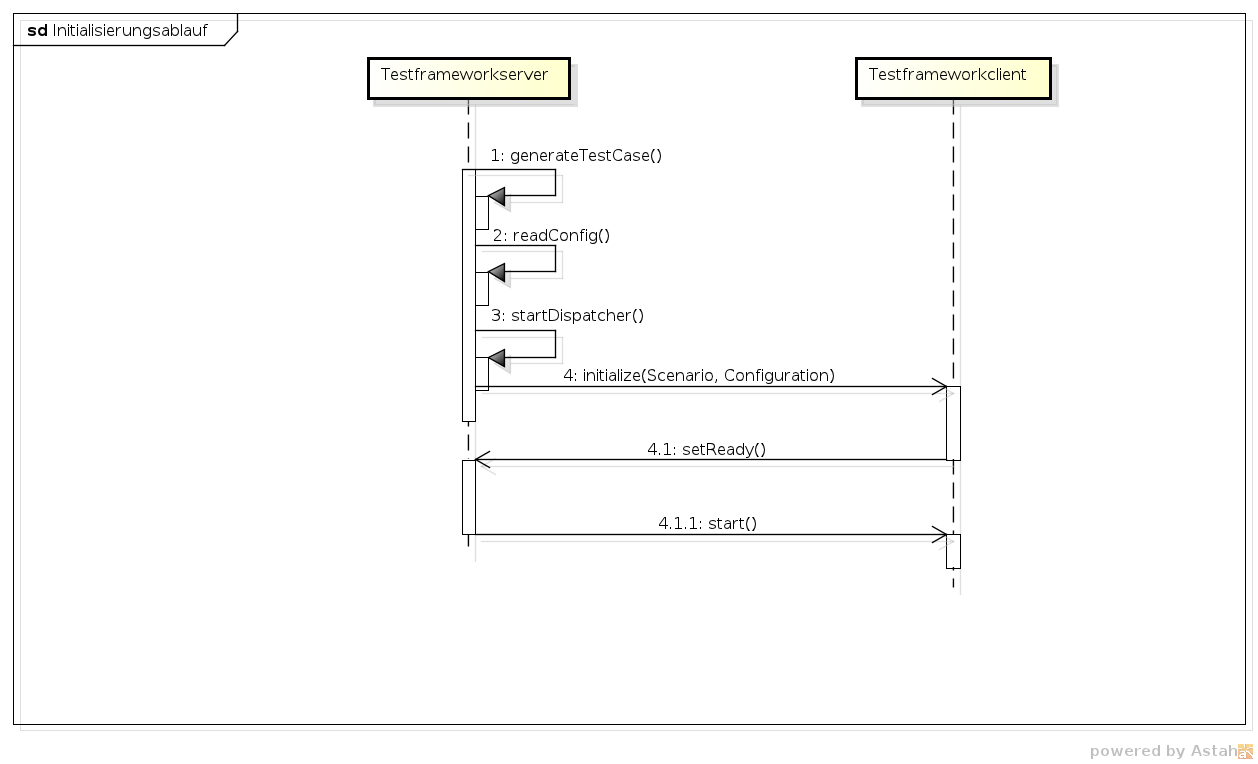
\includegraphics[scale=0.3]{image_testFramework/TestFWInit.png}
\end{center}

Die im Diagramm dargestellten Operationen lassen sich wie folgt erklären:

\begin{itemize}
\item Die Methode generateTestCase() ruft eine Factory auf, welche aus einer XML-Datei einen Testcase generiert. Diese Factory wird unter dem Kapitel Testcase-Factory genauer beschrieben.
\item Alle Konfigurationsparameter welche der Server braucht, sind in einer Konfigurationsdatei abgelegt. Durch eine Configurationfactory wird durch mit Hilfe der Konfigurationsdatei ein Configuration-Objekt erzeugt. Unter dem Kapitel "Configuration-Factory" wird dies näher beschrieben.
\item Nachdem die Konfigurationsparameter ausgelesen wurden, kann der Dispatcher in einem seperaten Thread gestartet werden. Weitere Ausführungen sind unter dem Kapitel "Der Dispatcher" zu finden.
\item Bei der Initialisierung der Clients, wird diesen je ein Scenario und ein Configuration-Objekt gesendet. Das Configuration-Objekt umfasst alle für den Client wichtigen Konfigurationsparameter, wie etwa die Ports, unter welchen der Server seine Dienste zur Verfügung stellt. Was ein Scenario genau ist wird unter dem "Kapitel Testcase-Factory" genauer beschrieben.
\item Pro Client hat der Server beim Auslesen der Konfigurationsdatei ein Client-Objekt instanziert. Dies wurde vorallem zur Kontrolle der Clients durch den Server so implementiert. Darauf wird im Kapitel "ClientObjekt" eingegangen.
\item Nachdem alle Clients "setReady()" aufgerufen haben, ruft der Server "start()" auf allen Clients auf. Diese beginnen dann mit dem eigentlichen Testlauf. Dadurch sichert der Server einen fairen Start des Testlaufs, da es ansonsten vorkommen könnte, dass einer der Clients massiv früher starten kann, als der andere.
\end{itemize}

\subsubsection{Testcase-Factory}
\label{sec:testCaseFactory}
Die Testcase-Factory liest ein XML-File, in welchem ein sogenannter "TestCase" definiert ist. Wird beim Starten des Frameworkservers kein Paramter mitgegeben, wird der Standard-Testcase gewählt, welcher in der Datei "testCases.xml" abgelegt ist. Wird aber ein Parameter mitgegeben, beschreibt dieser den Namen der auszuführenden TestCase-Datei.\newline
Durch die eingelesenen Informationen erstellt die Factory die Szenarien, welche dann weiter an die verschiedenen Clients gesendet werden. Folgender Block ist ein Auszug aus einer TestCase-Datei:

\begin{lstlisting}
<?xml version='1.0' encoding='UTF-8'?>
<TestRun>
  <TestCase SystemUnderTest="ch.hsr.objectCaching.rmiOnlyClient.RMIonlyClientSystem">
    <Account balance="1"></Account>
      <Scenario id="1">
        <ActionSequence>
          <Increment count ="100" delay="0" factor="1.1"></Increment>
	</ActionSequence>
      </Scenario>
      <Scenario id="2">
	<ActionSequence>
          <Increment count ="100" delay="0" factor="1.1"></Increment>
	</ActionSequence>
      </Scenario>
  </TestCase>
</TestRun>
\end{lstlisting}

Eine TestCase-Datei beschreibt genau einen TestCase. Ein TestCase kann verschiedene Szenarien beinhalten, oder aber auch nur ein Szenario beschreiben. Ist nur ein Szenario definiert, werden beide Clients mit demselben Szenario arbeiten. Falls mehrere Szenarien beschrieben sind, werden die Clients unterschiedliche Szenarien durchführen. \newline
Ein Szenario besteht aus einer Abfolge von verschiedenen Actions. Was genau eine Action ist, ist unter dem Kapitel "Actions" erläutert.


\subsubsection{Configuration-Factory}
\label{sec:configurationFactory}

\subsubsection{Der Dispatcher}
\label{sec:dispatcher}

\subsubsection{ClientObjekt}
\label{sec:ClientObjekt}


\begin{itemize}	

\item Resultate \& Auswertung
\item Für die Beweisführung das Lost Updates nicht mehr möglich sind, musste ein zusätzlicher Listener eingebaut der die event protokoliert.
\end{itemize}

\subsection{Testframework Client}
\label{sec:test-FW Client}
Dieses Kapitel beschreibt die Aufgaben der Testframework Client Komponenten und deren Umsetzung. Der Testframework Clients hat zwei Hauptaufgaben, als erstes erzeugt und konfiguriert er das benötigte ClientSystemUnderTest. Zweitens muss er auf einem ClientSystemUnderTest eine gegebens Szenerio abarbeiten können. Die Umsetzung des Testframeworks haben wir über das bewährte Client/Server Konzepts realisiert, was zu einer schlanke Lösung auf Seiten des Clients führte. Dadurch lässt sich der Framework Client und das ClientSystemUnderTest direkt vom Framework Server aus konfigurieren und steuern. Ein weiterer Vorteil liegt darin das sich neue Anforderungen jederzeit leicht umsetzen lassen.


\subsubsection{ClientController}
\label{sec:clientController}

\begin{center}
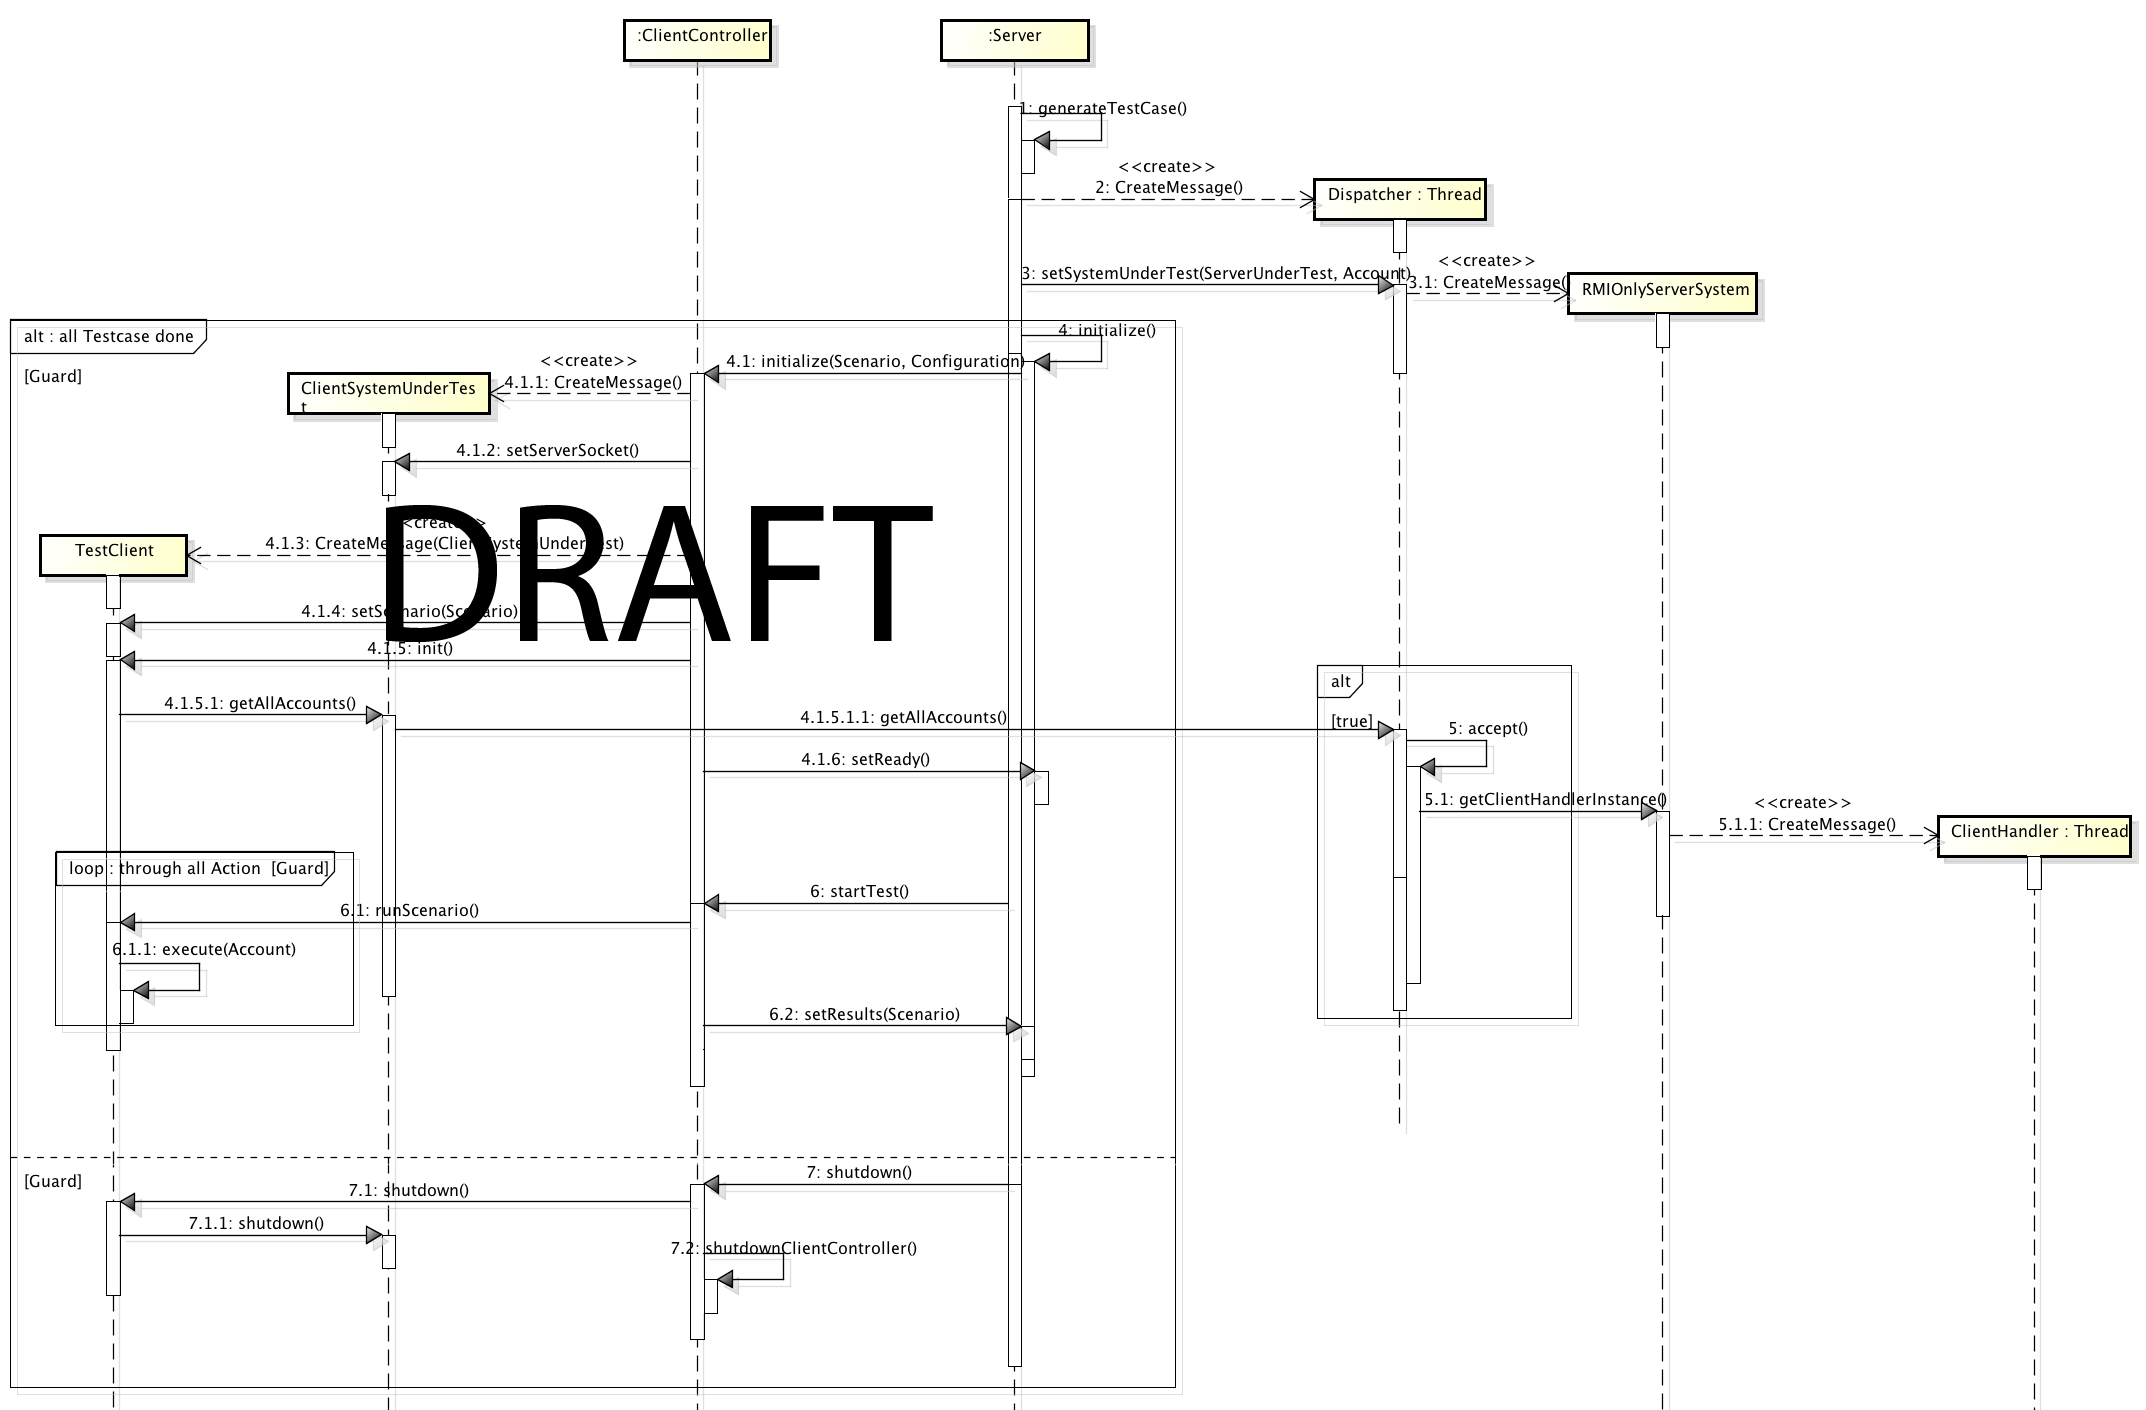
\includegraphics[scale=0.2]{image_testFramework/TestFWServerClientSeq.png}
\end{center}
 
Die Kommunikation zwischen den Testframework Clients und dem Server haben wir über Java RMI realisiert. Beim Start eines Testframework Clients wird ein neuer ClientController instanziiert, daraufhin wird dieses Objekt zur Java RMI Runtime exportiert. Die Veröffentlichung, das ClientController- Objekts erledigt die RMI Runtime im Hindergrund, ist das Objekt erfolgreich unter dem Namen, der als Argument beim start des ClientController mitgegeben wurde registriert, lässt sich der ClientController über Remote Method Invocation vom Server steuern. Der Port auf der die RMI Registry Anfragen akzeptiert lässt sich ebenfalls via Argument mitgeben falls keine Portnummer mitgegeben wird, wird der Defaultport 1099 verwendet.

Folgendes Interface wird vom ClientController implementiert und lässt sich über Java RMI benutzen:
\begin{lstlisting}[language=java, breaklines=true] 	
public void initialize(Scenario scenario, Configuration configuration) throws RemoteException;
public void startTest() throws RemoteException;
public void shutdown() throws RemoteException;
\end{lstlisting}
Über dieses Interface lässt sich der gesamte Testprozess des Clients steuern. Zu Beginn wollten wir die einzelnen Konfigurationswerte als Parameter übergeben, wir merkten jedoch schnell das es sinnvoller wäre einen neuen Datentypen einzuführen, der die alle benötigten Parameter für die Konfiguration des ClientSystemUnderTest sowie des ClientController beinhaltet und die Werte kapselt. Dieses Konfiguration beinhaltet unter anderem den Namen des ClientSystemUnderTest sowie die nötigen Information für den erfolgreichen Aufbau der RMI Kommunikation zwischen dem Testframework Client und dem Testframework Server. In der initialize() Methode wird als erstes ein Server Stub geladen. Zweitens, wird aus dem Configuration Objekt das gewünschte ClientSystemUnderTest herausgelesen und via Reflection instanziiert. Die Instanziierung des konkreten ClientSystemUnderTest wird in einer seperaten Factory erledigt. Danach wird ein neues TestClient-Objekt mit dem zuvor erzeugten CUT erzeugt. Als letztes wird der TestClient wird mit dem gegeben Szenario initialisiert. Sind alle Vorbereitungsschritte abgeschlossen, wird der Server über die erfolgreiche Initialisierung des CUT und des ClientController informiert. Der Server startet den Testdurchlauf parallel auf allen ClientController über die Methode startTest(). Sind alle Aktionen des gegeben Szenarios abgearbeitet, wird das gesamte Szenario mit den enthaltenen Messresultaten zurück an den Server geschickt, dort wird die Auswertung der Resultate vom Server übernommen. Der Testframework Client sowie das ClientSystemUnderTest laufen in derselben Java Virtual Machine um für jeden Testlauf dieselben JVM Umgebung zu gewährleisten, haben wir uns dazu entschlossen, bei jedem Testcase das ganze System neu zu starten. Über die Methode shutdown() lässt sich daher der Testframework Client sowie der CUT herunterfahren. Die shutdown() Methode löscht das Binding zwischen dem spezifischen Namen und dem damit verbundenen Objekt. Danach wir das Objekt von der RMI Runtime entfernt. Ist dies erledigt beendet sich der ClientController selbst. Beim testen der shutdown() Funktionalität merken wir schnell das, wenn wir dies wie oben beschrieben umsetzten, dass der Server eine Exception bekommt, dies lag daran das der ClientController zu schnell die Verbindung zum Server beendet hat, so dass der Server keine Zeit fand seine RMI Verbindung zum ClientController zu schliessen. Als Lösung des Problems verzögern wir nun die Beendigung (System.exit()) des ClientController um zwei Sekunden. Die Beendigung des ClientController wird in einem seperaten Thread ausgeführt, sodass der main Thread noch genügend Zeit hat, alle offenen Verbindungen ordnungsgemäss zu schliessen.    

\subsubsection{Test Client}
\label{sec:testclient}
Die Klasse TestClient ist die Schnittstelle zwischen dem Testframework und dem ClientSystemUnderTest. Im Konstruktor dieser Klasse kann ein Objekt übergeben werden, welches das ClientSystemUnderTest Interface implementiert. Startet der Server den Testlauf wird im TestClient das zuvor gesetzte Szenario abgearbeitet. Hierfür wird auf jedem Aktion Objekt die Methode execute(Account accunt) aufgerufen. Das Account Objekt, welches der execute Methode übergeben werden muss, wird aus der List von Accounts die von AccountService bereitgestellt wird geholt und übergeben.(Ringbuffer). Bei einem Shutdown durch den Server ist der TestClient ebenfalls für die ordnungsgemässe Beendigung des ClientSystemUnderTest zuständig.

\subsubsection{Action}
\label{sec:action}
Ein Szenario beinhaltet eine Menge von Aktionen die auf ein Account Objekt ausgeführt werden können. Für eine einfache Erweiterbarkeit von neuen Aktionen haben wir hierfür das Command-Pattern genutzt. Alle konkreten Implementierung von Aktionen leiten von der abstrakte Klasse Action ab. Im Konstruktor  dieser abstrakten Klasse wird ein neues Result Objekt instanziert. Dieses Objekt dient als Datenkontainer für alle Zeitmessungen die während dieser Aktion ausgeführt werden sollen. Desweiteren deklariert Action drei abstrakte Methoden die von Subklassen implementiert werden müssen.
 
\subsubsection{Increment Action}
\label{sec:incrementAction}
Um unsere Anforderungen abdenken zu können, benötigten wir nur die KontoErhöhen Aktion (IncrementAction), die den aktuellen Kontostand des Account Objekts holt (getBalance()) und den aktuellen Kontostand mit dem gegeben Faktor multipliziert und daraufhin den neuen berechneten Kontostand zurück in den Account schreibt(setBalance()). Zusätzlich war es nötig, dass zwischen der der getBalance() und der setBalance() eine minimal definierbare Zeitdauer gewartet werden kann. Diese Warteperiode ist nötig, damit sich leicht ein Konflikt erzeugen lässt und so gezeigt werden kann, dass der Fehler serverseitig zu keinem Lost-Updates führt. Tritt serverseitig ein Concurrency Fehler auf wird eine RuntimeExeption geworfen, dies führt auf der clientseite dazu, dass die ganze Aktion nochmals gestartet wird mit dem Unterschied das diesmal keine Verzögerung zwischen getBalance() und setBalance() vorkommt.

\subsubsection{Result}
\label{sec:result}
Für die Zeitmessung einer Aktion nutzen wir die von Java bereitgestellte Methode System.nanoTime(). Die Result Klasse bietet eine startTimeMeasurement() Methode die ein neues TimeRecord Objekt erzeugt und die momentane Zeit in das TimeRecord Objekt schreibt. (diese Methode verlangt eine BasicAction Typ der als Enum realisiert wurde(Erklärung warum nötig unter Resultate)). Über stopTimeMeasurement() lässt sich die aktuelle Messung beenden und der aktuelle TimeRecord wird abgelegt. Da innerhalb der execute() Methode mehrere setBalance() oder getBalance() möglich sind, muss es möglich sein mehrere TimeRecords pro Result Objekt zu erfassen.

\subsubsection{TimeRecord}
\label{sec:timeRecord}
Der TimeRecordtyp ist als reines Data Tranfer Object ausgelegt. Es beinhaltet die Startzeit sowie die Stopzeit genau einer Aktion. Für einen genauen Auswertung einer Aktion sind noch weiter Daten nötig. Daher besitzt dieser Typ zwei weiter Felder. Der BasicActiontyp beinhaltet Informationen für welche Methode dieser Record gilt und das ActionResult speichert die Information über den Erfolg der BasicAction. Dadurch lassen sich zusammengesetzte Aktion, welche aus getBalance() und setBalance() zusammengesetzt sind unterteilen. 




